\chapter{Analysis}

\section{Introduction}

\subsection{Client Identification}
My client is Ian Vines. He works for the company Huxley Bertram which is an engineering company that focuses on designing and making machines for other companies. He is involved in designing the machines and checking which parts are available and getting the ones that aren't.
\subsection{Define the current system}
There is currently no organised system for the task provided. The current system is a text document that is not organised. All the data in the document is not in a structured form and some of the data in the document may not be updated as to update the data would require manually adjusting it.
\subsection{Describe the problems}
The company currently gets machine parts from all different companies and people and at the moment the only information they have about the companies is on the text doument. To find out what company they get a certain machine part from they have to go through all the pages to find the right one. This takes a lot of time and they need a system that can make the process a lot quicker.
\subsection{Section appendix}

\section{Investigation}

\subsection{The current system}
A text document/Notepad with the information that is needed to buy the part from the company. It usually consists of the company's name, address, email, phone number, postcode, website name, part name and part price.

\subsubsection{Data sources and destinations}

\begin{center}
\begin{tabular}{ |c|c|c| } 
\hline
\bf\underline{Data}                                                                                                      & \bf\underline{Data Source} & \bf\underline{Data Destination}

\\
\hline
\ Company Address & Email & Document\\ 
\hline
\ Company Information & Email & Document\\
\hline
\ Part Required Information & Company Website & Document\\
\hline
\ Part Required Price & Company Website & Document\\
\hline
\end{tabular}
\end{center}
\subsubsection{Algorithms}

search document
if part name is part looking for
get company information
else
keep looking

\subsubsection{Data flow diagram}
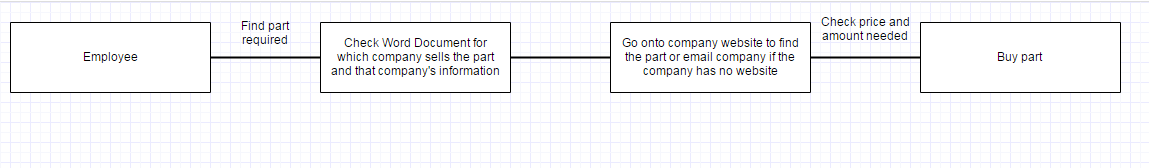
\includegraphics{Flowchart.png}


\subsection{The proposed system}
The proposed system will be a database that stores all of the different company's information and which machine part they are selling. The program will allow you to add or remove companies from the database according to any new information you receive. It will also allow you to edit the information stored in the data base allowing you to update any changes that may have happened. You will also be allowed to search key words such as a company's name or the specific part you need. The program will then show all the appropriate companies with the part you need,the price and the company's contact information. The program will also show the comments of other employees on what they thought of the product and if it suited their needs.

\subsubsection{Data sources and destinations}
\begin{center}
\begin{tabular}{ |c|c|c| } 
\hline
\bf\underline{Data}                                                                                                      & \bf\underline{Data Source} & \bf\underline{Data Destination}

\\
\hline
\ Company Address & Email & Database\\ 
\hline
\ Company Information & Email & Database\\
\hline
\ Part Required Information & Company Website & Database\\
\hline
\ Part Required Price & Company Website & Database\\
\hline
\end{tabular}
\end{center}
\subsubsection{Algorithms}

\underline{Search for part}
if part is same as part searched for
output company information
elif
if part is not the same as part seaarched for
do not display
else
part is not valid

\underline{Adding a part}
while confirm is no
output please enter a part and the corresponding company information
input part and information
output confirm
if confirm is yes
add to database
else 
confirm is no

\underline{Deleting a part}
while confirm is no
output please enter a part to remove
input part
output confirm
if confirm is yes
delete from database
else 
confirm is no

\subsubsection{Data flow diagram}

\subsubsection{Data dictionary}
\begin{center}
\begin{tabular}{ | m{2cm} | m{2cm} | m{2cm} | m{3cm} | m{3cm} | } 
\hline
\underline{\bf Name}& \bf\underline{Data Type} & \bf\underline{Length} & \bf\underline{Validation} & \bf\underline{Example}

\\
\hline
\ Company Name & String & Unlimited & Make sure the data is a string and not any other data type & The Name Company\\ 
\hline
\ Company Address & String and Integer & 0 to 26 characters & Maximum of 26 characters, Information is actually there and it is a string with integers & Example Address\\
\hline
\ Company Phone Number & Integer & 11 integers & Make sure the input is not blank and is correct data type & 01234 567890\\
\hline
\ Company Email & String & Unlimited characters & No blank input. Data is correct data type & 123@example.com\\
\hline
\ Company Website & String & Unlimited characters & No blank input. Data is correct data type & www.example.com\\
\hline
\ Part Price & float & Unlimited characters & No blank input. Data is correct data type & £9.99\\
\hline
\ Part Name & String & Unlimited characters & No blank input. Data is correct data type & Screw\\
\hline
\end{tabular}
\end{center}
\subsubsection{Volumetrics}
The system should be able to store 200 company's information along with the part and price. It should allow for expansion to allow more information to be stored. 

\section{Objectives}

\subsection{General Objectives}
\begin{itemize}
	\item Menu must be easy to use and interact with
	\item The search must function quickly and must be easy to use
	\item The information stored must be easy to retrieve and access
	\item The company shown must be relevant to the part required
\end{itemize}

\subsection{Specific Objectives}
\begin{itemize}
	\item The user is able to edit the information 
	\item The price of the part is shown
	\item The Rating of the part is shown
	\item Employees can add comments about certain parts and companies
	\item Database can hold over 20 attributes
\end{itemize}
\subsection{Core Objectives}
\begin{itemize}
	\item The user is able to edit the information 
	\item The price of the part is shown
	\item The Rating of the part is shown
	\item Employees can add comments about certain parts and companies
\end{itemize}
\subsection{Other Objectives}
\begin{itemize}
	\item able to print information
	\item able to delete information
\end{itemize}
\section{ER Diagrams and Descriptions}

\subsection{ER Diagram}

\subsection{Entity Descriptions}

\section{Object Analysis}

\subsection{Object Listing}
\begin{itemize}
	\item employee
	\item Part Needed
	\item Company information
\end{itemize}

\subsection{Relationship diagrams}

\subsection{Class definitions}
\bf\underline{Employee}
\begin{itemize}
	\item First Name
	\item Last Name
	\item ID 
\end{itemize}
\bf\underline{Part Needed}
\begin{itemize}
	\item Part Name
	\item Part Size
	\item Part Price
\end{itemize}
\bf\underline{Company Information}
\begin{itemize}
	\item Company Name
	\item Company Email
	\item Company Telephone number
	\item Company Website
	\item Company Owner
\end{itemize}
\section{Other Abstractions and Graphs}

\section{Constraints}

\subsection{Hardware}
The hardware available is the basic computer hardware. This includes: A mouse, A keyboard, A monitor, A computer, Speakers. Anything else is not available as not every employee has the hardware.

\subsection{Software}
The software available mut be downloadable (if needed) and must be available to Windows 7,8 and 10.
\subsection{Time}
The deadline is april
\subsection{User Knowledge}
The system must be simple and easy to use by someone who is not familiar with all the functions on a computer. It must have a layout that is easy to access the information and has everything that is needed within one window. There shouldn't be multiple windows open.
\subsection{Access restrictions}
Every employee should be allowed to use the software so there are no access restrictions.

\section{Limitations}

\subsection{Areas which will not be included in computerisation}

\subsection{Areas considered for future computerisation}

\section{Solutions}

\subsection{Alternative solutions}
\bf \underline{Spreadsheet}
\\
\bf {Advantages}
\begin{itemize}
	\item Can hold all of the information about each company and each part
	\item Can be stored as a table
	\item Can add/remove data
\end{itemize}
\bf {Disadvantages}
\begin{itemize}
	\item Can't search for a specific part
	\item Not easy to find information
	\item Will not prioritise parts according to review left by other employees
	\item May need specific program downloaded
\end{itemize}
\bf \underline{Database}
\\
\bf {Advantages}
\begin{itemize}
	\item Can hold all of the information about each company and each part
	\item Can be searched for specific items
	\item Can filter searches to user specifications 
	\item Can add/remove data
	\item Can hold a wide range of data
\end{itemize}
\bf {Disadvantages}
\begin{itemize}
	\item May need specific program downloaded
	\item Limited to interface
	\item Limited to features included
\bf \underline{Writing a Program}
\\
\bf {Advantages}
\begin{itemize}
	\item Can Include a database if needed
	\item Can Customise to include a whole range of features
	\item Can Filter searches to user specifications 
	\item Can Add/remove data
	\item Can Create a simple and easy to use interface
\end{itemize}
\bf {Disadvantages}
\begin{itemize}
	\item May need specific program downloaded
	\item Can take time to write
	\item Can contain lots of errors if done incorrectly
\end{itemize}
\subsection{Justification of chosen solution}